\scanpage{79}
In the proof, essential use is made of the Hilbert polynomial, in fact we get a solution as a disjoint sum of subschemes of $S$ corresponding to various Hilbert polynomials. Still I would expect that the \deleted{\unsure{solution}} functor is representable as soon as $X/S$ is proper. In view of the application we have in mind here, it would be sufficient (for an\unsure{\deleted{y}|y} integral $S$) to findin $S$ a non empty \deleted{\unsure{set}} open set $S_1$ such Problem A has always a solution for $X_1=X\mathbin{x}_S S_1$ over $S_1$ . To prove this weeker existence result, it is well possible that a reduction to the projective case is possible, using Chow's lemma and some induction on the relative \unsure{dimension} perhaps. I also would expect that a proof will be easier when working over a complete noetherian local ring, hence the case of a general \begin{minipage}[c]{3.9cm}
\figure{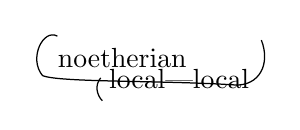
\begin{tikzpicture}[x=1cm,y=1cm,baseline=(word.base)]
\node[anchor=base west,inner sep=0pt] at (-0.65,0.27) {\inserted{noetherian}};
\node[anchor=base west,inner sep=0pt] (word) at (0,0) {\unsure{local|\deleted{local}}};
\draw[line width=0.45pt] (-0.65,0.67) .. controls (-0.83,0.77) and (-1.02,0.39) .. (-0.84,0.17) .. controls (-0.64,0.08) and (0.72,0.11) .. (1.61,0.05) .. controls (1.91,0.04) and (2.06,0.31) .. (1.94,0.62);
\draw[line width=0.45pt] (-0.10,0.14) .. controls (-0.18,0.05) and (-0.15,-0.08) .. (-0.08,-0.15);
\end{tikzpicture}}
\end{minipage} ring by flat descent. And it is well possible that, putting together two such partial results, a proof of the existence in general could be obtained. (I met with such difficulties allready time ago in a very \unsure{analoguous|analognous} non projective existence problem, which beside I did not solve so far !). This problem A has been met also by Hartshorne (a Harvard student), but I doubt he will work seriously on it. Thus \deleted{to}\handwritten{\unsure{J|I}} now wrote you in the hope you may be interested to have a try on this problem. As a general fact , our knowledge of non projective existence theorems is exceedingly poor, and I hope this will change eventually.

\noindent\hspace*{1.5em}Sincerely yours\hfill\handwritten{A Grothendieck}\par
% archive sheet number: 78
